\section{Data and Methodology}


\subsection{Methodology}
The data used in this report is based on reanalysis data, which is a combination of model simulations and observational data. The data comes from the ERA5 reanalysis produced by the European Centre for Medium-Range Weather Forecasts (ECMWF). ERA5 is a global atmospheric reanalysis that provides a physically consistent estimate of the state of the atmosphere by assimilating observational data into numerical weather models \citep{hersbach2020}. The horizontal resolution is $0.25\degr \times 0.25\degr$ and covers the period from 2012 to 2021 by monthly means. The data were processed using Python (xarray), and graphical plots were produced using matplotlib and cartopy to visualize regional patterns and seasonal variability in the Arctic region.


The reanalysis data has strengths in providing a comprehensive and continuous dataset that covers a long period of time and a wide range of variables. However, it also has limitations. The reanalysed data combine observations from various sources, including satellites, weather stations, aeroplanes, and buoys, however some regions, especially in the Arctic, have sparse observational coverage, which lead to a stronger dependence on the ones present such as satellites \citep{hersbach2020}. This can give rise to errors and biases such as measuring cloud cover, due to the white surface of the ice and snow leading to an overestimation of the cloud cover in the region \citep{hersbach2020}. Other more complex interactions, such the sea ice and atmospheric interaction, will then be heavily dependent on the simulation model's ability to capture these interactions. Thus, the uncertainties from the model simulations can be higher due to lack of observations. Another important aspect to consider is temporal resolution. The data used in this report is based on monthly mean fields, which means that it may not capture short-term variability in the Arctic region such as storms or cyclones. 



\newpage

\subsection{The data}
Above in the background section two main sub-regions of the Arctic were defined, the Arctic dessert and the Arctic tundra. It is therefore relevant to evaluate the precipitation in the region, as it is a key factor in determining the type of ecosystem present. The annual mean precipitation for the period 2012 to 2021 can be seen in \autoref{fig:TotalPrecipitation_2012_2021_annual}. The figure shows that the Arctic region is generally dry, with most areas receiving less than \SI{1}{\mm} of precipitation per month. Higher levels of precipitation are observed in the tundra areas to the south. Thus categorizing the High Arctic as a dessert is reasonable, as it receives very little precipitation. 

In \autoref{fig:SeaSurfaceTemperature_2012_2021_annual} one can observe the annual mean sea surface temperature for the period. The figure shows warmer water temperatures reaching the arctic ocean near Fram Strait. One can also observe that the sea surface temperature is generally warmer near the Nordic Countries and the Barents Sea. However, places such as Baffin Bay, Arctic Archipelago, and the High Arctic the temperature is generally near or below freezing. 


\begin{figure}[H]
    \centering
    \begin{subfigure}[b]{0.49\textwidth}
        \centering
        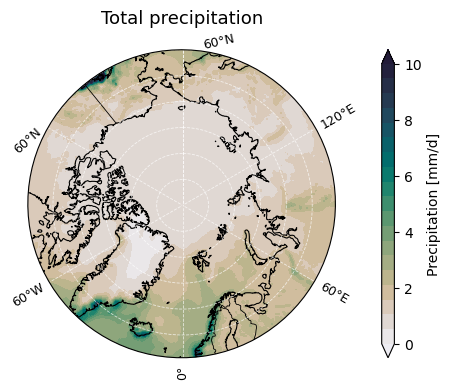
\includegraphics[height=0.23\textheight,keepaspectratio]{Figures/TotalPrecipitation_2012_2021_annual.png}
        \caption{Total Monthly Precipitation}
        \label{fig:TotalPrecipitation_2012_2021_annual}
    \end{subfigure}
    \hfill
    \begin{subfigure}[b]{0.49\textwidth}
        \centering
        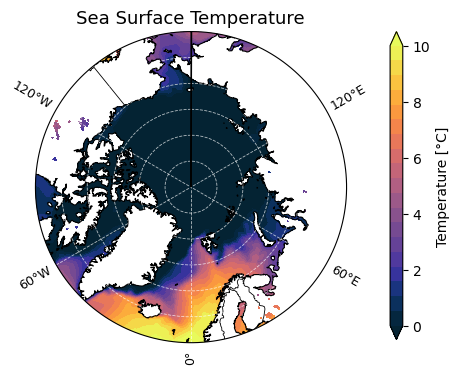
\includegraphics[height=0.23\textheight,keepaspectratio]{Figures/SeaSurfaceTemperature_2012_2021_annual.png}
        \caption{Sea Surface Temperature}
        \label{fig:SeaSurfaceTemperature_2012_2021_annual}
    \end{subfigure}
    \caption{Annual monthly mean total precipitation and sea surface temperature for 2012--2021.}
    \label{fig:annual_means}
\end{figure}

In \autoref{fig:annual_means} the annual mean was calculated, since the annual precipitation and sea surface temperature were interesting to observe to evaluate the type of ecosystem present in the region. However for the data in \autoref{fig:Temperature_2012_2021_mean}--\ref{fig:SeaIce_2012_2021_mean} the seasonal mean was calculated to evaluate the seasonal variability in the region. The seasonal mean was calculated by averaging the monthly mean fields for each season, where DJF corresponds to winter the months, MAM corresponds to the spring months, JJA corresponds to the summer months, and SON corresponds to the autumn months. This allows us to observe seasonal differences for variables such as temperature, sea level pressure, sea ice concentration, and boundary layer height, which all vary significantly across the seasons in the Arctic region. 

\newpage

The air temperature change throughout the seasons can be observed in \autoref{fig:Temperature_2012_2021_mean}. In the figure one can similar temperatures during the spring and the autumn, with slightly lower temperatures during the spring. The summer months are much warmer, with temperatures above freezing everywhere except for negative degrees in Greenland and zero degrees in the Arctic Ocean. The winter months are the coldest, with temperatures well below freezing across the entire region except the Norwegian Sea and parts of the Barents Sea. 


\begin{figure}[H]
    \begin{subfigure}[b]{0.49\textwidth}
        \raggedleft
        
\includegraphics[height=0.23\textheight,keepaspectratio]{Figures/Temperature_2012_2021_mean_DJF.png}
        \caption{DJF}
        \label{fig:Temperature_2012_2021_mean_DJF}
    \end{subfigure}
    \hfill
    \begin{subfigure}[b]{0.49\textwidth}
        \raggedright
        
\includegraphics[height=0.23\textheight,keepaspectratio]{Figures/Temperature_2012_2021_mean_MAM.png}
        \caption{MAM}
        \label{fig:Temperature_2012_2021_mean_MAM}
    \end{subfigure}
    \\[0.6em]
    \begin{subfigure}[b]{0.49\textwidth}
        \raggedleft
        
\includegraphics[height=0.23\textheight,keepaspectratio]{Figures/Temperature_2012_2021_mean_JJA.png}
        \caption{JJA}
        \label{fig:Temperature_2012_2021_mean_JJA}
    \end{subfigure}
    \hfill
    \begin{subfigure}[b]{0.49\textwidth}
        \raggedright
        
\includegraphics[height=0.23\textheight,keepaspectratio]{Figures/Temperature_2012_2021_mean_SON.png}
        \caption{SON}
        \label{fig:Temperature_2012_2021_mean_SON}
    \end{subfigure}
    \\[0.6em]
    \caption{Seasonal mean 2m air temperature (\degr C) for 2012--2021 for DJF, MAM, JJA, and SON.}
    \label{fig:Temperature_2012_2021_mean}
\end{figure}

The sea level pressure can be observed in \autoref{fig:SeaLevelPressure_2012_2021_mean}. The figure shows that the sea level pressure is generally very uniform during the summer months, with a slight high pressure system over Greenland. More interestingly is the winter months were a large pressure gradient can be observed between the low pressure system centred at Iceland, stretching up to southern Greenland, the Greenland Sea and the Barents Sea, and the high pressure system centred over the East Siberian Sea, but stretching over the entire Siberia and Canada. This indicate a strong cyclonic circulation during the winter months in the region.


\begin{figure}[H]
    \begin{subfigure}[b]{0.49\textwidth}
        \raggedleft
        
\includegraphics[height=0.23\textheight,keepaspectratio]{Figures/SeaLevelPressure_2012_2021_mean_DJF.png}
        \caption{DJF}
        \label{fig:SeaLevelPressure_2012_2021_mean_DJF}
    \end{subfigure}
    \hfill
    \begin{subfigure}[b]{0.49\textwidth}
        \raggedright
        
\includegraphics[height=0.23\textheight,keepaspectratio]{Figures/SeaLevelPressure_2012_2021_mean_MAM.png}
        \caption{MAM}
        \label{fig:SeaLevelPressure_2012_2021_mean_MAM}
    \end{subfigure}
    \\[0.6em]
    \begin{subfigure}[b]{0.49\textwidth}
        \raggedleft
        
\includegraphics[height=0.23\textheight,keepaspectratio]{Figures/SeaLevelPressure_2012_2021_mean_JJA.png}
        \caption{JJA}
        \label{fig:SeaLevelPressure_2012_2021_mean_JJA}
    \end{subfigure}
    \hfill
    \begin{subfigure}[b]{0.49\textwidth}
        \raggedright
        
\includegraphics[height=0.23\textheight,keepaspectratio]{Figures/SeaLevelPressure_2012_2021_mean_SON.png}
        \caption{SON}
        \label{fig:SeaLevelPressure_2012_2021_mean_SON}
    \end{subfigure}
    \\[0.6em]
    \caption{Seasonal mean sea level pressure (hPa) for 2012--2021 for DJF, MAM, JJA, and SON.}
    \label{fig:SeaLevelPressure_2012_2021_mean}
\end{figure}

The seasonal sea ice concentration can be observed in \autoref{fig:SeaIce_2012_2021_mean}. The figure shows that the sea ice concentration is generally very high during the winter and spring months, and much lower during the summer and autumn months. The sea ice concentration is higher in the High Arctic, but lower south of the Fram Strait and in Barents Sea. The most southern sea ice can be observed in the Bering Sea, where the sea ice concentration is around 0.5 during the winter months. More southern sea ice can be seen along the eastern coast of Greenland and in the Bering Strait. 


\begin{figure}[H]
    \begin{subfigure}[b]{0.49\textwidth}
        \raggedleft
        
\includegraphics[height=0.23\textheight,keepaspectratio]{Figures/SeaIce_2012_2021_mean_DJF.png}
        \caption{DJF}
        \label{fig:SeaIce_2012_2021_mean_DJF}
    \end{subfigure}
    \hfill
    \begin{subfigure}[b]{0.49\textwidth}
        \raggedright
        
\includegraphics[height=0.23\textheight,keepaspectratio]{Figures/SeaIce_2012_2021_mean_MAM.png}
        \caption{MAM}
        \label{fig:SeaIce_2012_2021_mean_MAM}
    \end{subfigure}
    \\[0.6em]
    \begin{subfigure}[b]{0.49\textwidth}
        \raggedleft
        
\includegraphics[height=0.23\textheight,keepaspectratio]{Figures/SeaIce_2012_2021_mean_JJA.png}
        \caption{JJA}
        \label{fig:SeaIce_2012_2021_mean_JJA}
    \end{subfigure}
    \hfill
    \begin{subfigure}[b]{0.49\textwidth}
        \raggedright
        
\includegraphics[height=0.23\textheight,keepaspectratio]{Figures/SeaIce_2012_2021_mean_SON.png}
        \caption{SON}
        \label{fig:SeaIce_2012_2021_mean_SON}
    \end{subfigure}
    \\[0.6em]
    \caption{Seasonal mean sea ice concentration (-) for 2012--2021 for DJF, MAM, JJA, and SON.}
    \label{fig:SeaIce_2012_2021_mean}
\end{figure}

